\SourcePage{705}{708}
\section{Regge poles}

Section~128 treated the scattering amplitude's analytic properties in the complex particle energy $E$, with orbital angular momentum $l$ serving as a parameter restricted to real integral values. Further properties of methodological importance emerge when $E$ is held real and $l$ is instead allowed to vary continuously as a complex variable\footnote{These properties were first investigated by Regge (T.~Regge, 1958).}.


\SourcePage{706}{709}
As in \S~128, consider radial wave functions whose asymptotic form as $r\to\infty$ is
\begin{equation}
 \chi_l=rR_l=A(l,E)\exp\left(-\frac{\sqrt{-2mE}}{\hbar}r\right)
 +B(l,E)\exp\left(\frac{\sqrt{-2mE}}{\hbar}r\right).
 \tag{141.1}
\end{equation}
These functions solve the Schrödinger equation (32.8), in which $l$ is now regarded as a complex parameter; one of the two independent solutions is selected by the condition
\begin{equation}
 R_l\approx\mathrm{const}\cdot r^l\quad\text{as }r\to0.
 \tag{141.2}
\end{equation}

This condition restricts the allowed values of $l$. The general form of a solution of (32.8) at small $r$ is
\[
 R_l\approx c_1r^l+c_2r^{-l-1}
\]
(see the end of \S~32). For the second solution to be distinguished unambiguously against the background of the first and excluded, $r^{-l-1}$ must be larger than $r^l$ as $r\to0$. For complex $l$ this gives $\Re l>\Re(-l-1)$, or
\begin{equation}
 \Re\left(l+\frac12\right)>0.
 \tag{141.3}
\end{equation}
We henceforth consider this half-plane of complex $l$, to the right of $l=-1/2$.

As a solution of a differential equation with coefficients analytic in $l$, $R(r;l,E)$ is analytic in this parameter and has no singularities in (141.3). This applies to (141.1), so $A(l,E)$ and $B(l,E)$ have no singularities in $l$. Retention of both terms of (141.1) as $r\to\infty$ is understood to be legitimate. For $E>0$ this is always so; for $E<0$ it holds if $U(r)$ satisfies (128.6) or (128.13). The asymptotic behaviour in $r$ depends only on $E$, not on $l$, so complex $l$ does not alter the conditions for reaching the asymptotic form.

Comparison with (128.15) gives
\begin{equation}
 S(l,E)=\exp[2i\delta(l,E)]=e^{i\pi l}\frac{A(l,E)}{B(l,E)},
 \tag{141.4}
\end{equation}

\SourcePage{707}{710}
also for complex $l$, although the phase shift $\delta$ is then not real.

For real $l$ and $E>0$, (128.4) gives $A(l,E)=B^*(l,E)$. Hence for complex $l$
\begin{equation}
 A(l^*,E)=B^*(l,E)\quad\text{for }E>0,
 \tag{141.5}
\end{equation}
and $S(l,E)$ satisfies \emph{complex unitarity}:
\begin{equation}
 S^*(l,E)S(l^*,E)=1.
 \tag{141.6}
\end{equation}

Because $A(l,E)$ and $B(l,E)$ have no singularities as functions of $l$, the only singularities (poles) of $S(l,E)$, and hence of the partial scattering amplitude $f(l,E)$, occur at zeros of $B(l,E)$. Poles of the scattering amplitude in the complex $l$-plane are termed \emph{Regge poles}. Their locations naturally depend on the value of the real parameter $E$. The functions $l=\alpha_i(E)$ that specify these locations are termed \emph{Regge trajectories}: as $E$ varies, the poles follow definite curves in the $l$-plane (below we shall omit the index $i$ that labels the poles).


We first show that for $E<0$ all $\alpha(E)$ are real. Consider
\begin{equation}
 \chi''+\left[\frac{2m}{\hbar^2}(E-U)-\frac{\alpha(\alpha+1)}{r^2}\right]\chi=0.
 \tag{141.7}
\end{equation}
Multiplying by $\chi^*$, integrating over $dr$, and integrating the first term by parts gives
\[
 -\int_0^\infty|\chi'|^2dr+\frac{2m}{\hbar^2}\int_0^\infty(E-U)|\chi|^2dr
 -\alpha(\alpha+1)\int_0^\infty\frac{|\chi|^2}{r^2}dr=0.
\]
For $B=0$, the Regge-pole condition, the wave function decreases exponentially as $r\to\infty$, so all integrals converge. The first two terms and the integral in the last term are real. Therefore
\[
 \Im[\alpha(\alpha+1)]=\Im\left(\alpha+\frac12\right)^2
 =2\Re\left(\alpha+\frac12\right)\Im\alpha=0.
\]

\SourcePage{708}{711}
Since only poles in (141.3) are considered, $\Re(\alpha+1/2)>0$, and
\begin{equation}
 \Im\alpha(E)=0\quad\text{for }E<0.
 \tag{141.8}
\end{equation}

Differentiate (141.7) with respect to $E$, multiply the result by $\chi$, multiply (141.7) by $\partial\chi/\partial E$, and subtract. This gives
\[
 \left[\chi'\frac{\partial\chi}{\partial E}-\chi\left(\frac{\partial\chi}{\partial E}\right)'\right]'
 -\frac{2m}{\hbar^2}\chi^2+\frac{\chi^2}{r^2}\frac{d\alpha(\alpha+1)}{dE}=0.
\]
Integration over $dr$ from 0 to $\infty$, using again the vanishing of $\chi$ at infinity, yields
\begin{equation}
 \frac{d\alpha(\alpha+1)}{dE}\int_0^\infty\frac{\chi^2}{r^2}dr
 =\frac{2m}{\hbar^2}\int_0^\infty\chi^2dr.
 \tag{141.9}
\end{equation}
Since $\alpha$ and the wave function are real, both integrals are positive. Thus
\[
 \frac{d\alpha(\alpha+1)}{dE}=2\left(\alpha+\frac12\right)\frac{d\alpha}{dE}>0,
\]
and, since $\alpha+1/2>0$,
\[
 \frac{d\alpha}{dE}>0\quad\text{for }E<0.
\]
Thus $\alpha(E)$ increases monotonically with $E$ for $E<0$.

Negative energies at which $\alpha(E)$ takes physical values, the integers $l=0,1,2,\ldots$, are discrete energy levels. This gives a new classification of bound states by the Regge trajectories on which they lie.

For example, in an attractive Coulomb field the scattering-matrix elements are\footnote{Compare (135.11), in which the signs before $k$ must be reversed in passing from repulsion to attraction.}
\begin{equation}
 S_l=\frac{\Gamma(l+1-i/k)}{\Gamma(l+1+i/k)}.
 \tag{141.10}
\end{equation}

\SourcePage{709}{712}
Here $k$ is in Coulomb units. The poles occur when the argument of $\Gamma(l+1-i/k)$ is a negative integer or zero. Since $k=i\sqrt{-2E}$ for $E<0$,
\begin{equation}
 \alpha(E)=-n_r-1+\frac1{\sqrt{-2E}},\qquad E<0,
 \tag{141.11}
\end{equation}
where $n_r=0,1,2,\ldots$ labels the trajectories. Setting $\alpha(E)=l=0,1,2,\ldots$ gives the Bohr formula
\[
 E=-\frac1{2(n_r+l+1)^2}.
\]
Here $n_r$ is the radial quantum number specifying the number of radial nodes. Each prescribed $n_r$, and hence each trajectory, corresponds to infinitely many levels distinguished by orbital angular momentum.

We turn to $\alpha(E)$ for $E>0$. Recall that $A(l,E)$ and $B(l,E)$, as functions of complex $E$, are defined on a plane cut along the positive real semiaxis. The roots $l=\alpha(E)$ of $B(l,E)=0$ have the same cut. On its two edges they take complex-conjugate values, with $\Im\alpha>0$ on the upper edge. We explain this by physical reasoning.

For complex $l$, the centrifugal energy and effective potential $U_l=U+l(l+1)/(2mr^2)$ are complex. Repeating the derivation of \S~19 gives
\[
 \frac{\partial}{\partial t}|\psi|^2+\operatorname{div}\mathbf j=2|\psi|^2\Im U_l.
\]
For $l=\alpha$ and $\Im\alpha>0$, one also has $\Im U_l>0$; the positive right-hand side is as though particles were emitted inside the field. The asymptotic wave function, containing only the first term of (141.1) when $B=0$, must accordingly be outgoing. This occurs on the upper edge of the cut; compare (128.1) and (128.3).

Since $\alpha(E)$ is complex for $E>0$, it cannot take physical values $l=0,1,$

\SourcePage{710}{713}
$2,\ldots$, but may approach them. We show that a resonance then appears in the corresponding partial amplitude.

Let $l_0$ be an integer near $\alpha(E)$, and let the positive real energy $E_0$ satisfy $\Re\alpha(E_0)=l_0$. Near it,
\begin{equation}
 \alpha(E)\approx l_0+i\eta+\beta(E-E_0),
 \tag{141.12}
\end{equation}
where $\eta=\Im\alpha(E_0)$ is real. On the upper edge, $\eta>0$, and proximity to $l_0$ means $\eta\ll1$. The constant $\beta=d\alpha/dE$ at $E_0$ can also be treated as real and positive. Since $\alpha$ is nearly real, $\chi(r;\alpha,E)$ is nearly real. Neglecting higher orders in $\eta$ and the imaginary part of $\chi$, positivity of $\beta$ follows from the positive integrals in (141.9)\footnote{To clarify these integrals, the asymptotic region $r\gg a$, where $a$ is the field range and (141.1) applies, contributes only slightly when $\eta$ is small. If $l=\alpha(E)$ is a zero of $B(l,E)$, then by (141.5) $l=\alpha^*$ is a zero of $A(l,E)$. Thus $A(\alpha,E)$, and hence $\chi(r;\alpha,E)$ for $r\gg a$, is of order $\eta^{1/2}$ (see (134.11)). On the upper edge of the cut the wave function contains $e^{ikr}$: $\chi(r;\alpha,E)=A(\alpha,E)e^{ikr}$. Taking $E$ as $E+i\delta$, $\delta\to+0$, gives $k$ a small positive imaginary part and ensures convergence of (141.9). Physically, the small contribution from $r\gg a$ reflects that $E_0$ is a quasistationary state; the particle reaches this region only through improbable decay. The main contribution comes from $r\sim a$, where the wave function is nearly real.}.

Because $l=\alpha(E)$ is a zero of $B(l,E)$, near $\alpha,E_0$ this function is proportional to $\alpha-l$. Hence
\begin{equation}
 B(l_0,E)\approx\mathrm{const}\cdot[\beta(E-E_0)+i\eta].
 \tag{141.13}
\end{equation}
This has the form (134.6), with energy $E_0$ and quasidiscrete-level width $\Gamma=2\eta/\beta>0$. Thus proximity of a Regge trajectory

\SourcePage{711}{714}
to integral $l$ at $E>0$ corresponds to quasistationary states. The same classification principle therefore applies as for stationary states: a trajectory may correspond to a family of discrete and quasidiscrete levels.

Complex $l$ gives a useful integral representation of the complete scattering amplitude for $E>0$, whose series is
\begin{equation}
 f(\mu)=\frac1{2ik}\sum_{l=0}^{\infty}(2l+1)[S(l,E)-1]P_l(\mu),\qquad\mu=\cos\theta.
 \tag{141.14}
\end{equation}

First define $P_l(\mu)$ for complex as well as integral $l$. Let it be the solution of (c.2)
\begin{equation}
 (1-\mu)^2P_l''(\mu)-2\mu P_l'(\mu)+l(l+1)P_l(\mu)=0
 \tag{141.15}
\end{equation}
with $P_l(1)=1$. As a function of $l$, it then has no finite singularities\footnote{Comparison with (e.2) expresses it through the hypergeometric function
\[
 P_l(\mu)=F\left(-l,l+1,1;\frac{1-\mu}{2}\right).
\]}.

The series (141.14) equals
\begin{equation}
 f(\mu)=\frac1{4k}\int_C\frac{2l+1}{\sin\pi l}[S(l,E)-1]P_l(-\mu)\,dl,
 \tag{141.16}
\end{equation}
where $C$ encircles clockwise all points $l=0,1,2,\ldots$ on the real axis and closes at infinity:

\begin{center}
\begin{tikzpicture}[x=1.1cm,y=0.8cm]
  \draw[->] (-1,0) -- (4.8,0);
  \foreach \x/\lab in {1/1,2/2,3/3,4/4}
    \draw (\x,0.09)--(\x,-0.09) node[below] {\lab};
  \draw (-0.5,0.09)--(-0.5,-0.09)
    node[below left,xshift=-1pt] {$-\tfrac12$};
  \draw (0,0.09)--(0,-0.09)
    node[below right,xshift=1pt] {$0$};
  \draw[->,rounded corners=6pt] (4.5,0.75)--(-0.2,0.75)--(-0.42,0)--(-0.2,-0.75)--(4.5,-0.75);
  \node[right] at (4.5,-0.75) {$C$};
\end{tikzpicture}
\end{center}

All poles $l=\alpha_1,\alpha_2,\ldots$ of $S(l,E)$, which for $E>0$ lie off the real axis, must remain outside $C$.

Indeed, (141.16) is $-2\pi i$ times the sum of residues of the integrand at $l=0,1,2,\ldots$, the poles of $1/\sin\pi l$, whose residues are $(-1)^l/\pi$. Since $P_l(-\mu)=(-1)^lP_l(\mu)$ for integral $l$, this reduces (141.16) to (141.14)\footnote{A fuller account of these topics in nonrelativistic theory is given in the book by de Alfaro and Regge cited in the note on p.~612.}.

\SourcePage{712}{715}
\subsection*{Problem}

Show that the phase shifts for successive integral $l$ satisfy
\[
 \delta_{l+1}(E)-\delta_l(E)<\pi/2.
\]

\SolutionHeading Regard $l$ as a continuous real variable and differentiate (32.10):
\[
 \left[\frac{\partial\chi}{\partial l}\right]''+\left[\frac{2m}{\hbar^2}(E-U)-\frac{l(l+1)}{r^2}\right]\frac{\partial\chi}{\partial l}
 =\frac{2l+1}{r^2}\chi.
\]
Multiply this equation by $\chi$, the original equation by $\partial\chi/\partial l$, and subtract:
\[
 \left[\chi\frac{\partial\chi'}{\partial l}-\chi'\frac{\partial\chi}{\partial l}\right]'
 =(2l+1)\frac{\chi^2}{r^2}.
\]
Integrate from 0 to $\infty$. At $r=0$ the bracket vanishes; at infinity use (33.20). Thus
\[
 4k\left(\frac\pi2-\frac{\partial\delta_l}{\partial l}\right)
 =(2l+1)\int_0^\infty\frac{\chi^2}{r^2}dr>0,
\]
so $\partial\delta_l/\partial l<\pi/2$. Integration from $l$ to $l+1$ gives the required inequality. Combined with (133.17), it proves that the number $n_l$ of discrete levels does not increase with $l$. At $E\to\infty$, where the Born approximation applies, $\delta_l(\infty)=0$. Hence
\[
 n_{l+1}-n_l=-\frac1\pi[\delta_{l+1}(0)-\delta_l(0)]<\frac12,
 \qquad n_{l+1}-n_l\le0.
\]
